\section{Resultados e discussão}\label{sec:resultados}

Esta seção apresenta os resultados obtidos com a plataforma computacional descrita na Seção~\ref{sec:metodologia}, aplicada a uma matriz de configurações de ponte de madeira roliça para estrada vicinal de pista simples. A matriz combina quatro vãos teóricos com as cinco classes de resistência de madeiras de florestas nativas da ABNT NBR 7190-3, mantendo fixos a largura da pista, o trem tipo e todos os coeficientes normativos, de modo que as diferenças observadas decorram exclusivamente do vão e da classe de resistência.

A apresentação está organizada em três blocos. O primeiro descreve a plataforma computacional desenvolvida (Seção~\ref{sec:plataforma}) e define a matriz de casos (Seção~\ref{sec:casos}). O segundo detalha exaustivamente uma célula de referência da matriz (Seção~\ref{sec:caso_detalhado}), na qual são exercitados todos os recursos analíticos da ferramenta: fronteira eficiente, comparação com amostragem aleatória, grau de utilização das verificações, custo da robustez, validação por simulação independente, convergência por hipervolume, sensibilidade global de Sobol e dispersão das variáveis de projeto. O terceiro percorre a matriz completa (Seção~\ref{sec:varredura}) e converte os resultados em ábacos de anteprojeto (Seção~\ref{sec:abacos}).

\subsection{Plataforma computacional}\label{sec:plataforma}

Como principal produto de engenharia deste trabalho, foi desenvolvida uma plataforma computacional de acesso livre para o dimensionamento de pontes de madeira, capaz de realizar a verificação completa dos elementos estruturais em conformidade com as ABNT NBR 7190 \parencite{NBR7190-1:2022} e NBR 7188 \parencite{nbr7188}, disponível nos idiomas português e inglês \parencite{ReliaBridge2026}. A interface, ilustrada nas Figuras~\ref{fig:tela_inicial} e~\ref{fig:interface_dim}, é organizada em módulos que permitem a navegação sequencial entre as etapas de dimensionamento por otimização, projeto detalhado dos elementos e análise dos resultados. Ao final do processamento, a ferramenta disponibiliza para download a planilha de dados de entrada, os resultados do pré-dimensionamento, as estatísticas descritivas das variáveis de projeto e as figuras geradas.

\begin{figure}[!ht]
    \centering
    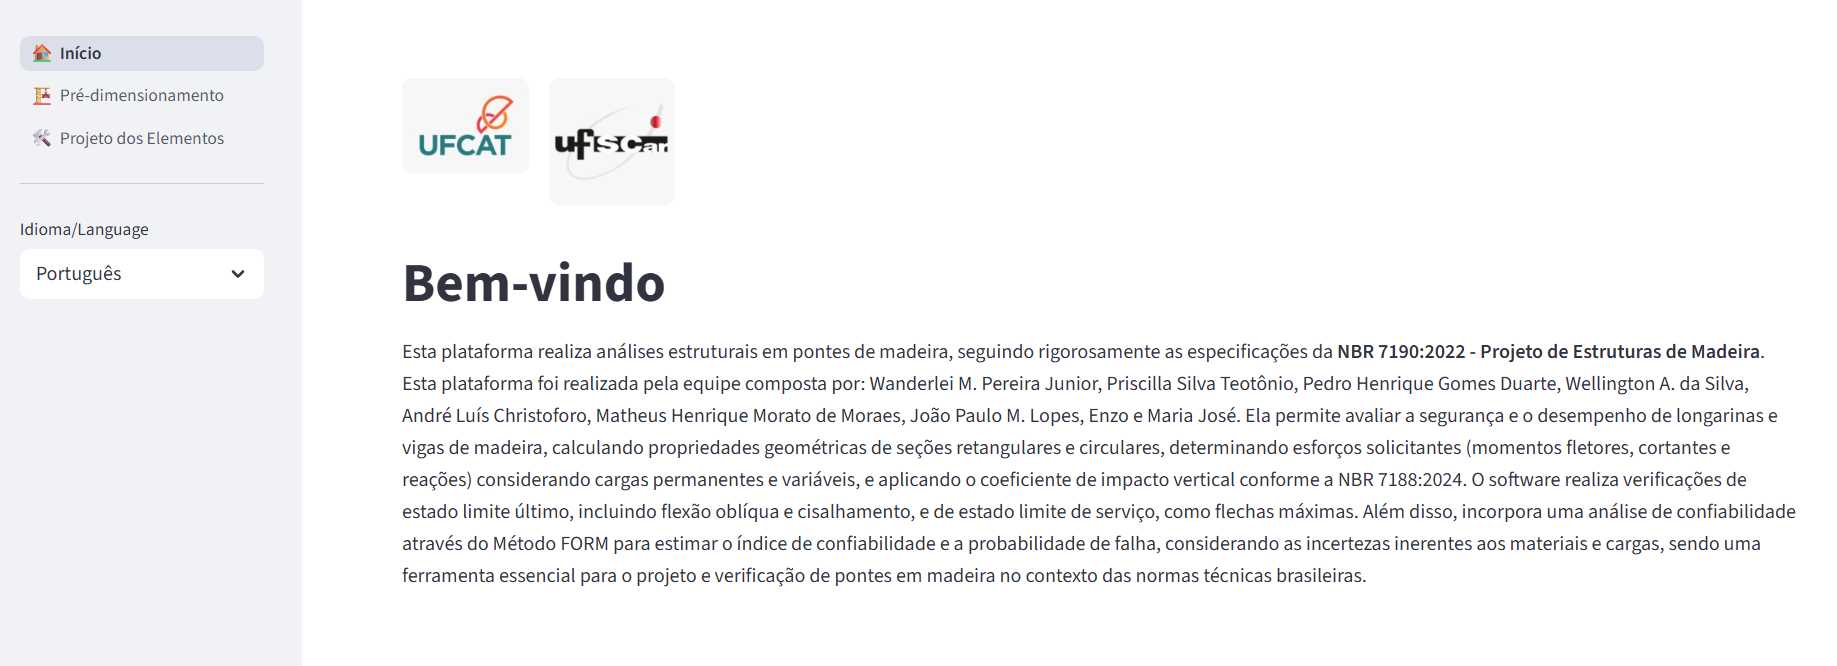
\includegraphics[width=0.85\textwidth]{figuras/interface_inicial.png}
    \caption{Tela inicial da plataforma computacional.}
    \label{fig:tela_inicial}
\end{figure}

\begin{figure}[!ht]
    \centering
    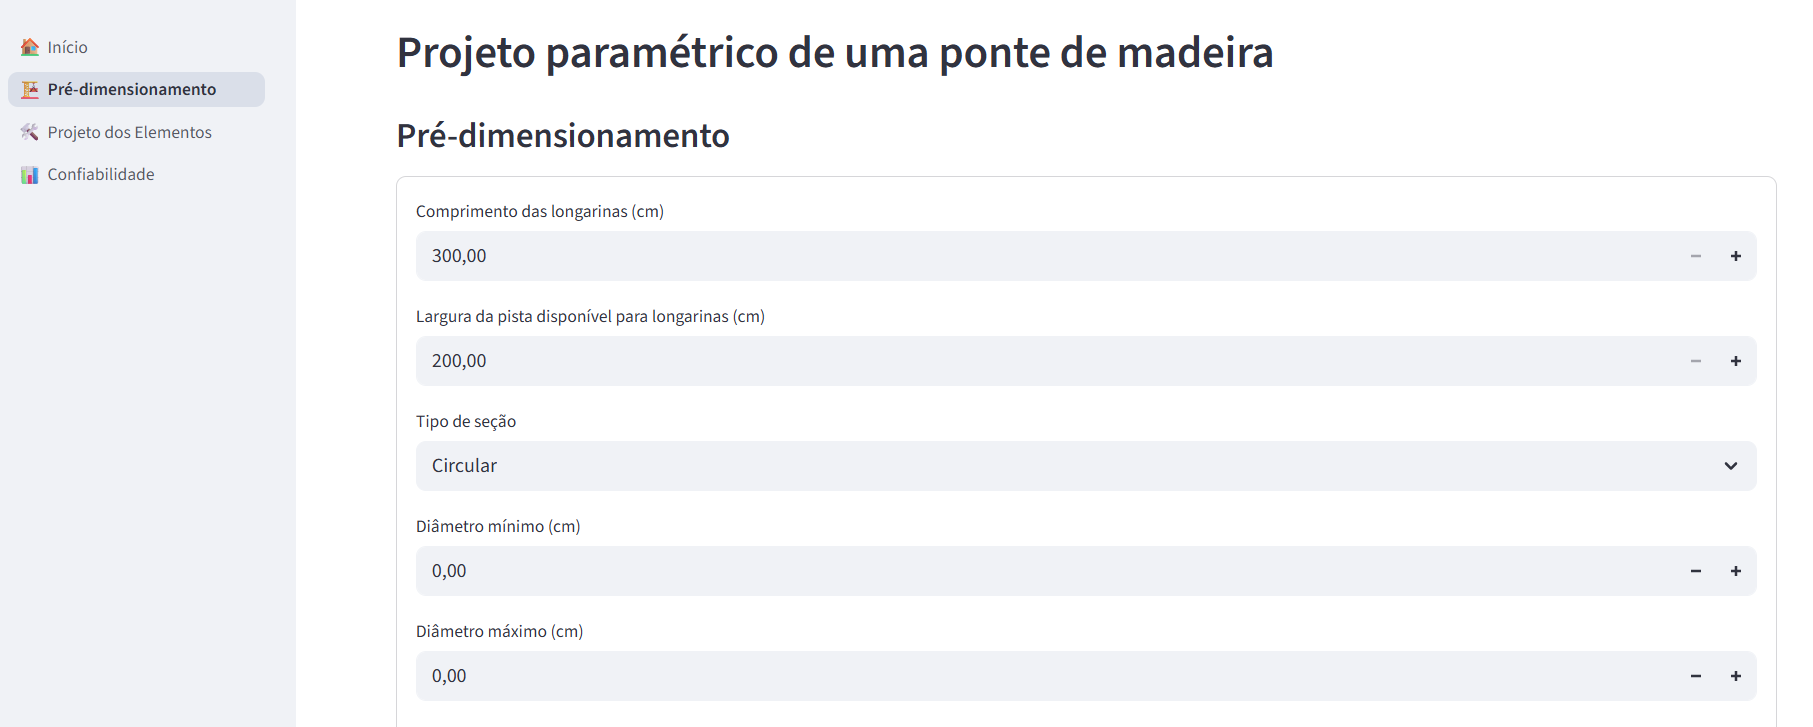
\includegraphics[width=0.9\textwidth]{figuras/interface_dimensionamento.png}
    \caption{Módulo de dimensionamento por otimização.}
    \label{fig:interface_dim}
\end{figure}

\subsection{Definição da matriz de casos de estudo}\label{sec:casos}

Os parâmetros geométricos, de carregamento e os coeficientes normativos mantidos constantes em toda a matriz são apresentados na Tabela~\ref{tab:parametros}. A largura de pista de 4{,}5~m corresponde à seção transversal usual de ponte vicinal de pista simples, compatível com o tráfego de um veículo por vez e com guarda-rodas laterais.

\begin{table}[!ht]
\caption{Parâmetros geométricos, de carregamento e coeficientes normativos comuns a toda a matriz.\label{tab:parametros}}
\begin{threeparttable}
\begin{tabular*}{\columnwidth}{@{\extracolsep\fill}lc@{\extracolsep\fill}}
\toprule
Parâmetro & Valor \\
\midrule
Largura da pista, $b_{w,\mathrm{pista}}$ (cm) & 450 \\
Trem tipo (ABNT NBR 7188) & TB-240 \\
Carga concentrada por roda, $p_{rodak}$ (kN) & 40 \\
Carga variável distribuída, $p_{qk}$ (kPa) & 4 \\
Carga permanente distribuída, $p_{gk}$ (kPa) & 1 \\
Distância entre eixos, $a$ (m) & 1{,}5 \\
Classe de carregamento & Permanente \\
Classe da madeira & Madeira natural \\
Classe de umidade & 1 \\
Coeficiente parcial das ações permanentes, $\gamma_g$ & 1{,}35 \\
Coeficiente parcial das ações variáveis, $\gamma_q$ & 1{,}50 \\
Coeficiente de minoração (tensões normais), $\gamma_{wf}$ & 1{,}40 \\
Coeficiente de minoração (cisalhamento), $\gamma_{wc}$ & 1{,}80 \\
Fator de combinação quase permanente, $\psi_2$ & 0{,}30 \\
Coeficiente de fluência, $\varphi$ & 0{,}60 \\
Desvio de robustez, $\rho$ (\%) & 5{,}0 \\
\bottomrule
\end{tabular*}
\begin{tablenotes}
\footnotesize
\item As propriedades mecânicas da madeira não constam desta tabela por variarem entre as células da matriz; são as da Tabela~\ref{tab:classes_madeira}, conforme a classe de resistência de cada célula.
\end{tablenotes}
\end{threeparttable}
\end{table}

A matriz de casos é o produto cartesiano de quatro vãos teóricos por cinco classes de resistência, totalizando vinte configurações, conforme a Tabela~\ref{tab:matriz}. A faixa de vãos de 3{,}0 a 6{,}0~m foi escolhida por dois motivos. O primeiro é de representatividade: corresponde à extensão usual dos cursos d'água transpostos por pontes de madeira roliça em vias vicinais. O segundo é de consistência de formulação: nesse intervalo o momento fletor devido à carga móvel é dado integralmente pela Equação~\eqref{eq:mqk30}, sem a parcela adicional de multidão da Equação~\eqref{eq:mqk45}, de modo que as curvas de resultado não apresentam descontinuidade de formulação.

\begin{table}[!ht]
\caption{Matriz de casos de estudo. Cada célula corresponde a uma execução independente do NSGA-II.\label{tab:matriz}}
\begin{threeparttable}
\begin{tabular*}{\columnwidth}{@{\extracolsep\fill}lccccc@{\extracolsep\fill}}
\toprule
 & \multicolumn{5}{c}{Classe de resistência (ABNT NBR 7190-3)} \\
\cmidrule{2-6}
Vão $L$ (m) & D20 & D30 & D40 & D50 & D60 \\
\midrule
3{,}0 & C-01 & C-02 & C-03 & C-04 & C-05 \\
4{,}0 & C-06 & C-07 & C-08 & C-09 & C-10 \\
5{,}0 & C-11 & C-12 & \textbf{C-13} & C-14 & C-15 \\
6{,}0 & C-16 & C-17 & C-18 & C-19 & C-20 \\
\bottomrule
\end{tabular*}
\begin{tablenotes}
\footnotesize
\item A célula C-13 ($L = 5{,}0$~m, classe D40), destacada em negrito, é adotada como caso de referência para a análise detalhada da Seção~\ref{sec:caso_detalhado}.
\end{tablenotes}
\end{threeparttable}
\end{table}

Os intervalos de busca das cinco variáveis de projeto, comuns a todas as células, são apresentados na Tabela~\ref{tab:intervalos}. Os limites foram estabelecidos de modo a abranger as dimensões comerciais usuais de madeira roliça e de pranchas serradas, sem restringir artificialmente o espaço de busca do algoritmo.

\begin{table}[!ht]
\caption{Intervalos adotados para as variáveis de projeto.\label{tab:intervalos}}
\begin{threeparttable}
\begin{tabular*}{\columnwidth}{@{\extracolsep\fill}lcc@{\extracolsep\fill}}
\toprule
Variável & Valor mínimo (cm) & Valor máximo (cm) \\
\midrule
Diâmetro da longarina, $d$ & 30 & 150 \\
Largura da prancha do tabuleiro, $b_w$ & 5 & 60 \\
Altura da prancha do tabuleiro, $h$ & 5 & 60 \\
Espaçamento entre longarinas, $esp_{long}$ & 30 & 200 \\
Espaçamento entre peças do tabuleiro, $esp_{tab}$ & 5 & 60 \\
\bottomrule
\end{tabular*}
\end{threeparttable}
\end{table}

\subsection{Caso de referência detalhado: $L = 5{,}0$~m, classe D40}\label{sec:caso_detalhado}

Esta seção exercita todos os recursos analíticos da plataforma sobre uma única célula da matriz, a C-13. A escolha recai sobre um vão intermediário e uma classe de resistência intermediária, de modo que o comportamento observado seja representativo do conjunto. Os resultados das demais dezenove células são reportados de forma condensada na Seção~\ref{sec:varredura}.

\subsubsection{Fronteira eficiente e soluções representativas}\label{sec:fronteira_ref}

A otimização robusta multiobjetivo da célula C-13, com $\rho = 5\%$, gerou um conjunto de soluções não dominadas distribuídas ao longo da fronteira eficiente, apresentada na Figura~\ref{fig:fronteira_ref}. A Tabela~\ref{tab:solucoes_ref} reúne uma amostra representativa dessas soluções, com as respectivas funções objetivo e o maior valor entre as seis funções limite, confirmando o atendimento aos critérios normativos mesmo sob a avaliação robusta.

\begin{figure}[!ht]
    \centering
    \includegraphics[width=0.6\textwidth]{figuras/fronteira_C13.png}
    \caption{Fronteira eficiente da célula de referência C-13 ($L = 5{,}0$~m, D40, $\rho = 5\%$).}
    \label{fig:fronteira_ref}
\end{figure}

\begin{table}[!ht]
\caption{Soluções representativas da fronteira eficiente da célula C-13.\label{tab:solucoes_ref}}
\begin{threeparttable}
\setlength{\tabcolsep}{3pt}
\begin{tabular*}{\textwidth}{@{\extracolsep{\fill}}cccccccc@{\extracolsep{\fill}}}
\toprule
$d$ (cm) & $b_w$ (cm) & $h$ (cm) & $esp_{long}$ (cm) & $esp_{tab}$ (cm) & $V_{\mathrm{total}}$ (m\textsuperscript{3}) & $\delta_{\mathrm{tot}}/(L/250)$ & $g_{\max}$ \\
\midrule
\tofill{--} & \tofill{--} & \tofill{--} & \tofill{--} & \tofill{--} & \tofill{--} & \tofill{--} & \tofill{--} \\
\tofill{--} & \tofill{--} & \tofill{--} & \tofill{--} & \tofill{--} & \tofill{--} & \tofill{--} & \tofill{--} \\
\tofill{--} & \tofill{--} & \tofill{--} & \tofill{--} & \tofill{--} & \tofill{--} & \tofill{--} & \tofill{--} \\
\tofill{--} & \tofill{--} & \tofill{--} & \tofill{--} & \tofill{--} & \tofill{--} & \tofill{--} & \tofill{--} \\
\tofill{--} & \tofill{--} & \tofill{--} & \tofill{--} & \tofill{--} & \tofill{--} & \tofill{--} & \tofill{--} \\
\tofill{--} & \tofill{--} & \tofill{--} & \tofill{--} & \tofill{--} & \tofill{--} & \tofill{--} & \tofill{--} \\
\tofill{--} & \tofill{--} & \tofill{--} & \tofill{--} & \tofill{--} & \tofill{--} & \tofill{--} & \tofill{--} \\
\bottomrule
\end{tabular*}
\begin{tablenotes}
\footnotesize
\item \tofill{[A PREENCHER] Selecionar de cinco a sete soluções da fronteira final, ordenadas do extremo de menor volume ao extremo de menor flecha adimensional, incluindo obrigatoriamente os dois extremos. $g_{\max}$ é o maior valor entre $g_1$ e $g_6$ da solução, e deve ser negativo ou nulo para que a solução seja viável.}
\end{tablenotes}
\end{threeparttable}
\end{table}

\begin{fillblock}
\noindent\textbf{[A PREENCHER]} Descrever a tendência observada ao longo da fronteira: a faixa de volume de madeira entre os dois extremos, em m\textsuperscript{3}, e o correspondente intervalo de flecha adimensional. Indicar qual das seis restrições permanece ativa ao longo da maior parte da fronteira, pois é ela que define a forma da curva. Comentar se existe algum trecho da fronteira em que a restrição ativa muda, o que se manifesta como uma mudança de curvatura.
\end{fillblock}

\subsubsection{Comparação com amostragem aleatória}\label{sec:mc_projeto}

Para demonstrar o ganho atribuível ao processo de otimização, gerou-se um conjunto de soluções por amostragem aleatória uniforme no domínio das variáveis de projeto, sem qualquer estratégia de busca dirigida, retendo-se apenas as realizações que satisfazem simultaneamente as seis restrições. A Figura~\ref{fig:mc_ref} sobrepõe essa nuvem de soluções viáveis à fronteira eficiente obtida pelo NSGA-II.

\begin{figure}[!ht]
    \centering
    \includegraphics[width=0.6\textwidth]{figuras/fronteira_vs_mc_C13.png}
    \caption{Comparação entre a fronteira eficiente e as soluções viáveis obtidas por amostragem aleatória, célula C-13.}
    \label{fig:mc_ref}
\end{figure}

\begin{fillblock}
\noindent\textbf{[A PREENCHER]} Reportar o número total de amostras geradas e o número de amostras viáveis, com a respectiva taxa de viabilidade. Discutir a comparação: a dispersão das soluções aleatórias no espaço objetivo e a posição da fronteira de Pareto em relação a essa nuvem. Quantificar o ganho, escolhendo dois ou três níveis de flecha adimensional e comparando, para cada nível, o volume de madeira da melhor solução aleatória contra o da solução correspondente da fronteira. Essa é a comparação que sustenta a afirmação de que a otimização não é um refinamento marginal.
\end{fillblock}

\subsubsection{Grau de utilização das verificações normativas}\label{sec:utilizacao}

A Figura~\ref{fig:utilizacao} apresenta o grau de utilização de cada verificação normativa para uma solução selecionada da fronteira, entendido como a razão entre solicitação e resistência, no caso dos estados limites últimos, ou entre deslocamento e limite admissível, no caso do estado limite de serviço. O valor de 100\% corresponde ao limite normativo. Essa figura complementa o memorial de verificação reproduzido no Apêndice~\ref{ap:relatorio}.

\begin{figure}[!ht]
    \centering
    
\includegraphics[width=0.75\textwidth]{figuras/utilizacao_C13.png}
    \caption{Grau de utilização de cada verificação normativa para a solução selecionada da fronteira robusta da célula C-13.}
    \label{fig:utilizacao}
\end{figure}

\begin{fillblock}
\noindent\textbf{[A PREENCHER]} Gerar a figura como gráfico de barras horizontais, uma barra por verificação: flexão da longarina, cisalhamento da longarina, flecha da longarina e flexão do tabuleiro, com o grau de utilização em porcentagem no eixo horizontal e uma linha vertical de referência em 100\%. Discutir qual verificação está mais próxima do limite, isto é, qual governa o dimensionamento, e qual apresenta a maior folga. Relacionar esse resultado com o valor de $g_{\max}$ da mesma solução na Tabela~\ref{tab:solucoes_ref}: as duas informações devem ser consistentes.
\end{fillblock}

\subsubsection{Custo da robustez}\label{sec:custo_robustez}

A otimização determinística tende a posicionar as soluções ótimas exatamente sobre a fronteira das restrições ativas, tornando-as sensíveis a pequenas variações nas variáveis de projeto. Em pontes de madeira roliça, essa sensibilidade é agravada pela variabilidade natural do diâmetro das peças e pelas tolerâncias de fabricação e montagem. A incorporação da robustez desloca a fronteira eficiente para o interior do domínio viável: enquanto a otimização determinística tende a produzir soluções com função limite de flexão da longarina praticamente nula ($g_1 \approx 0$), a otimização robusta penaliza essas soluções, pois sob perturbação de $\pm\rho$ parte das realizações resultaria em violação.

Para quantificar esse efeito, a célula C-13 foi reotimizada para quatro níveis de desvio, $\rho \in \{0\%,\ 2{,}5\%,\ 5\%,\ 10\%\}$, mantendo inalterados todos os demais parâmetros do algoritmo (Tabela~\ref{tab:nsga2}). O caso $\rho = 0\%$ corresponde à otimização determinística, com $N_c = 1$, e serve de referência.

\begin{figure}[!ht]
    \centering
    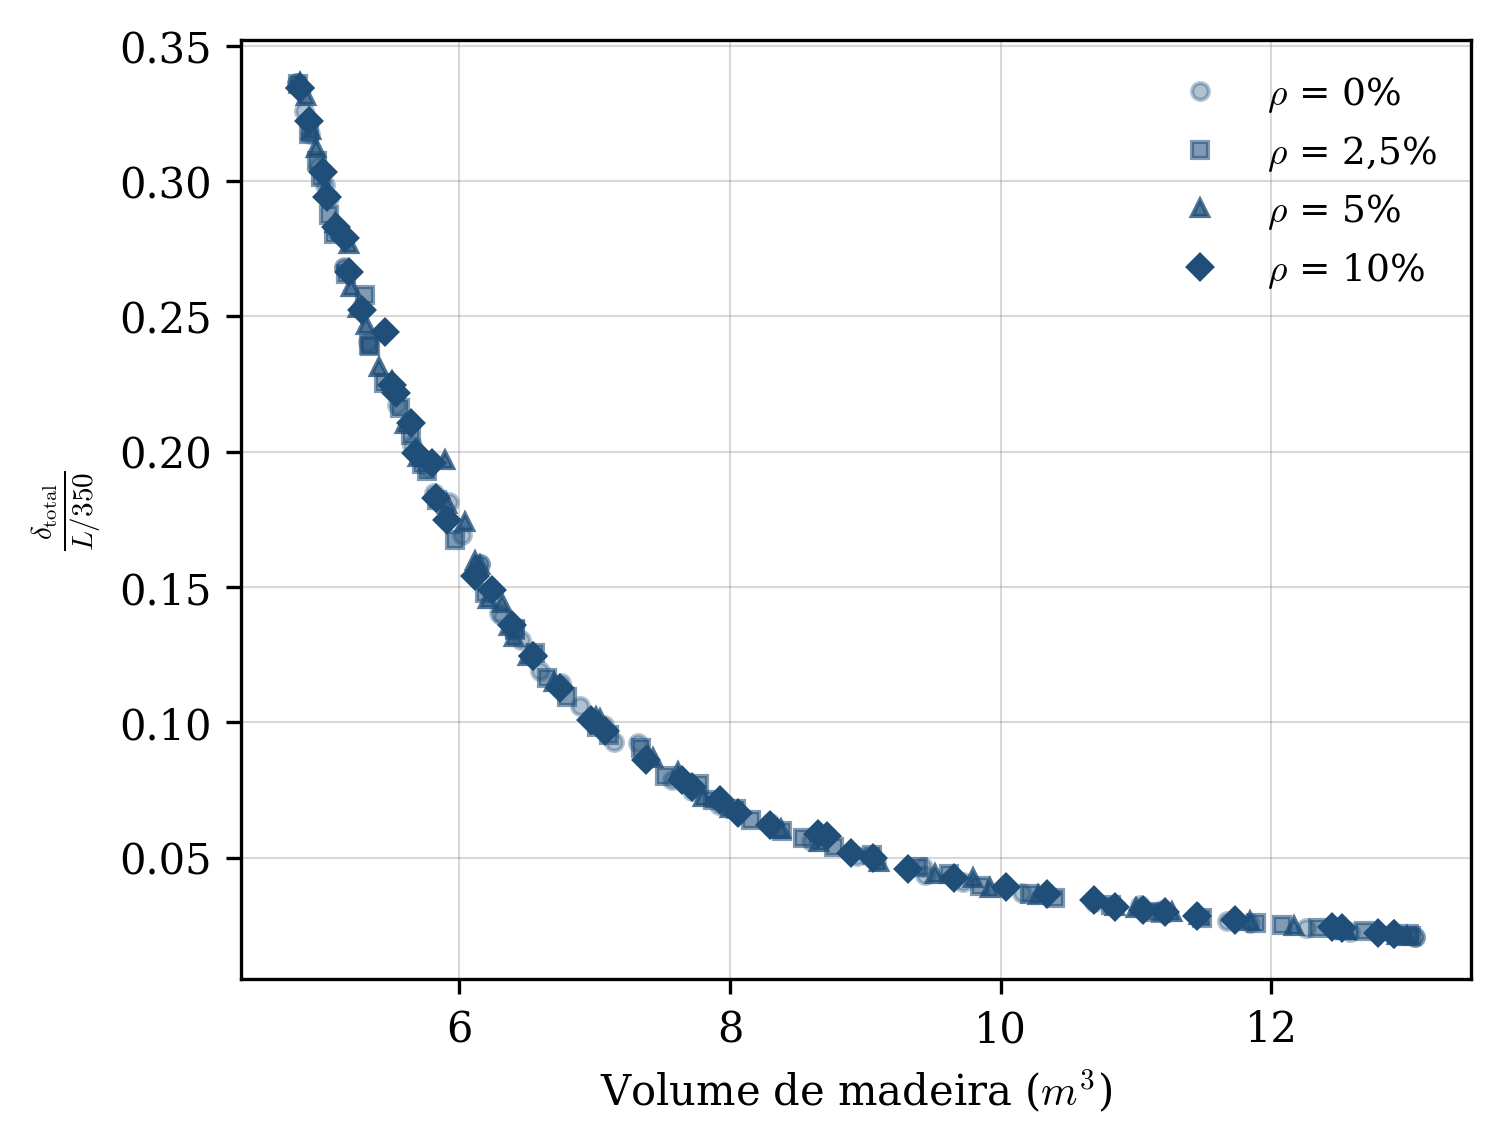
\includegraphics[width=0.7\textwidth]{figuras/custo_robustez_C13.png}
    \caption{Fronteiras eficientes da célula C-13 para $\rho = 0\%$, $2{,}5\%$, $5\%$ e $10\%$.}
    \label{fig:custo_robustez}
\end{figure}

\begin{table}[!ht]
\caption{Acréscimo percentual de volume de madeira em relação ao caso determinístico ($\rho = 0\%$), para três níveis pareados de flecha adimensional.\label{tab:custo_robustez}}
\begin{threeparttable}
\setlength{\tabcolsep}{3pt}
\begin{tabular*}{\columnwidth}{@{\extracolsep\fill}lccccccc@{\extracolsep\fill}}
\toprule
$\delta_{\mathrm{tot}}/(L/250)$ & $V(0\%)$ & $V(2{,}5\%)$ & $\Delta$ & $V(5\%)$ & $\Delta$ & $V(10\%)$ & $\Delta$ \\
\midrule
\tofill{--} & \tofill{--} & \tofill{--} & \tofill{--\%} & \tofill{--} & \tofill{--\%} & \tofill{--} & \tofill{--\%} \\
\tofill{--} & \tofill{--} & \tofill{--} & \tofill{--\%} & \tofill{--} & \tofill{--\%} & \tofill{--} & \tofill{--\%} \\
\tofill{--} & \tofill{--} & \tofill{--} & \tofill{--\%} & \tofill{--} & \tofill{--\%} & \tofill{--} & \tofill{--\%} \\
\bottomrule
\end{tabular*}
\begin{tablenotes}
\footnotesize
\item Volume em m\textsuperscript{3}; $\Delta$ é o acréscimo percentual em relação a $V(0\%)$ para o mesmo nível de flecha adimensional.
\end{tablenotes}
\end{threeparttable}
\end{table}

\begin{fillblock}
\noindent\textbf{[A PREENCHER]} Discutir a Figura~\ref{fig:custo_robustez} e a Tabela~\ref{tab:custo_robustez}. Verificar se o deslocamento da fronteira para o interior do domínio viável é monotônico em $\rho$ e se o acréscimo de volume cresce de forma aproximadamente linear ou acelerada com o nível de desvio. Reportar o tempo de processamento de cada uma das quatro execuções, informação que revisores da área de otimização costumam solicitar. Concluir de forma explícita quanto material adicional custa cada nível de tolerância a desvios dimensionais: este é o resultado de maior originalidade do trabalho e merece uma frase conclusiva quantificada.
\end{fillblock}

\subsubsection{Validação por simulação de Monte Carlo independente}\label{sec:validacao_mc}

Para verificar empiricamente o ganho de robustez, selecionou-se uma solução da fronteira determinística ($\rho = 0\%$) e uma solução de volume equivalente da fronteira robusta ($\rho = 5\%$), ambas da célula C-13. Para cada uma delas, geraram-se $10^4$ realizações perturbadas segundo $\tilde{\mathbf{x}} = \mathbf{x}\,(1+\rho\,\boldsymbol{\xi})$, com $\boldsymbol{\xi}\sim\mathcal{U}(-1,1)$ e semente aleatória distinta da utilizada durante a otimização, avaliando-se o percentual de realizações que violam cada uma das seis restrições, bem como a probabilidade de violação do sistema, entendida como a violação de ao menos uma restrição.

\begin{table}[!ht]
\caption{Percentual de realizações perturbadas que violam cada restrição ($10^4$ amostras, $\rho = 5\%$).\label{tab:validacao_mc}}
\begin{threeparttable}
\begin{tabular*}{\columnwidth}{@{\extracolsep\fill}lcc@{\extracolsep\fill}}
\toprule
Restrição & Solução determinística & Solução robusta \\
\midrule
$g_1$ -- flexão da longarina & \tofill{--\%} & \tofill{--\%} \\
$g_2$ -- cisalhamento da longarina & \tofill{--\%} & \tofill{--\%} \\
$g_3$ -- flecha da longarina & \tofill{--\%} & \tofill{--\%} \\
$g_4$ -- flexão do tabuleiro & \tofill{--\%} & \tofill{--\%} \\
$g_5$ -- espaçamento entre longarinas & \tofill{--\%} & \tofill{--\%} \\
$g_6$ -- espaçamento entre peças do tabuleiro & \tofill{--\%} & \tofill{--\%} \\
\midrule
Sistema (ao menos uma violação) & \tofill{--\%} & \tofill{--\%} \\
\bottomrule
\end{tabular*}
\end{threeparttable}
\end{table}

\begin{fillblock}
\noindent\textbf{[A PREENCHER]} Discutir a Tabela~\ref{tab:validacao_mc} com atenção a dois pontos. Primeiro, como a formulação adotada agrega as restrições pela média (Seção~\ref{sec:robustez}), é esperado que a solução robusta ainda viole a restrição mais ativa em uma fração não desprezível das realizações; reportar esse valor sem atenuá-lo é mais convincente do que omiti-lo, e abre caminho para a discussão de agregação por pior caso nas conclusões. Segundo, a linha ``Sistema'' é a comparação mais relevante para o projetista, pois considera todos os modos de violação simultaneamente. Certificar-se de que a semente utilizada nesta validação é efetivamente distinta da semente da otimização, sob pena de a validação ser circular.
\end{fillblock}

\subsubsection{Qualidade da fronteira: hipervolume e convergência}\label{sec:hipervolume}

A qualidade de uma fronteira aproximada é avaliada, de forma independente da inspeção visual, pelo indicador de hipervolume ($HV$), que mede a fração do espaço objetivo dominada pela fronteira em relação a um ponto de referência $\mathbf{r}$, conforme a Equação~\eqref{eq:hv} \parencite{blank2020}.

\begin{equation}
HV(\mathcal{F}_1, \mathbf{r}) = \mathrm{Vol}\left(\bigcup_{\mathbf{x} \in \mathcal{F}_1} \left[f_1(\mathbf{x}), r_1\right] \times \left[f_2(\mathbf{x}), r_2\right]\right)
\label{eq:hv}
\end{equation}

A Figura~\ref{fig:convergencia_hv} apresenta a evolução do hipervolume em função do número de gerações, justificando a posteriori o número de gerações adotado na Tabela~\ref{tab:nsga2}. Os valores finais do indicador, o \textit{spacing} da fronteira e a geração em que o hipervolume se estabiliza são reunidos na Tabela~\ref{tab:hv}, para os quatro níveis de robustez avaliados.

\begin{figure}[!ht]
    \centering
    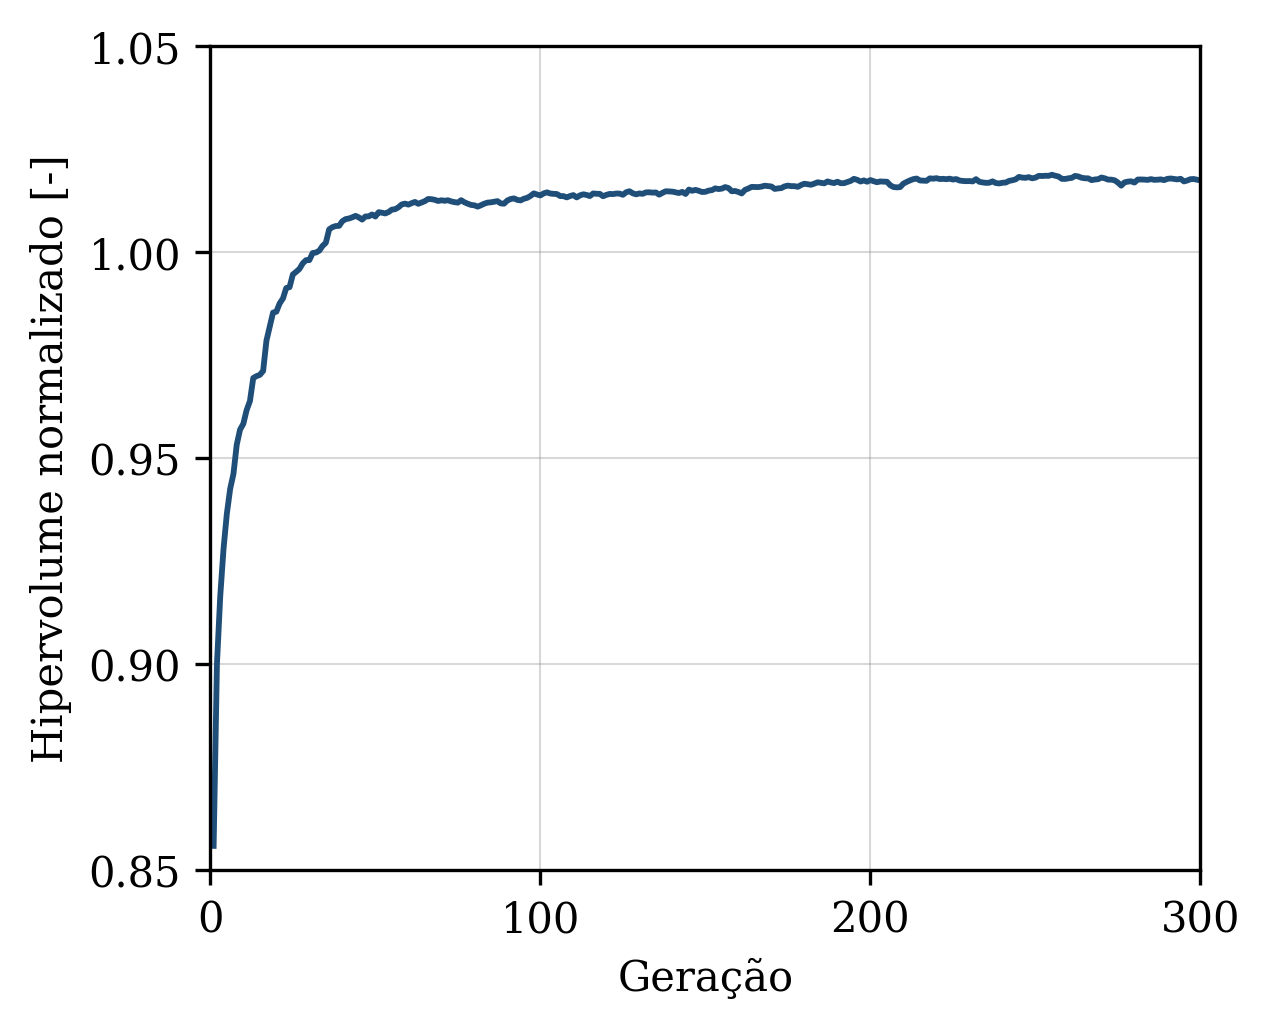
\includegraphics[width=0.7\textwidth]{figuras/convergencia_hv.png}
    \caption{Evolução do hipervolume ao longo das gerações do NSGA-II.}
    \label{fig:convergencia_hv}
\end{figure}

\begin{table}[!ht]
\caption{Hipervolume final, \textit{spacing} e geração de estabilização por nível de robustez.\label{tab:hv}}
\begin{threeparttable}
\begin{tabular*}{\columnwidth}{@{\extracolsep\fill}lcccc@{\extracolsep\fill}}
\toprule
Célula & $\rho$ (\%) & $HV$ & \textit{Spacing} & Geração de estabilização \\
\midrule
C-13 & 0{,}0 & \tofill{--} & \tofill{--} & \tofill{--} \\
C-13 & 2{,}5 & \tofill{--} & \tofill{--} & \tofill{--} \\
C-13 & 5{,}0 & \tofill{--} & \tofill{--} & \tofill{--} \\
C-13 & 10{,}0 & \tofill{--} & \tofill{--} & \tofill{--} \\
\bottomrule
\end{tabular*}
\begin{tablenotes}
\footnotesize
\item Ponto de referência $\mathbf{r}$: \tofill{[A PREENCHER -- definir e declarar explicitamente, por exemplo 10\% acima do pior valor observado em cada objetivo, após normalização pelos pontos ideal e nadir.]}
\end{tablenotes}
\end{threeparttable}
\end{table}

\begin{fillblock}
\noindent\textbf{[A PREENCHER]} Comentar se o hipervolume estabiliza antes do número de gerações adotado, o que justifica o custo computacional escolhido, e como o \textit{spacing} varia com $\rho$. Espera-se que fronteiras mais robustas sejam mais curtas no espaço objetivo, o que pode reduzir o \textit{spacing} mesmo mantendo boa diversidade; se for esse o caso, explicitar a distinção entre extensão e uniformidade da fronteira para evitar leitura equivocada do indicador.
\end{fillblock}

\subsubsection{Análise de sensibilidade global por índices de Sobol}\label{sec:sobol}

Para identificar quais variáveis de projeto mais influenciam a violação de cada restrição sob perturbação, realizou-se uma análise de sensibilidade global pelo método de Sobol \parencite{Sobol2001}, implementado na biblioteca \texttt{UQpy} \parencite{Olivier2020}. Os índices de efeito total $S_{T_i}$ das cinco variáveis de projeto foram estimados em relação às seis funções limite, a partir de uma amostragem independente de $N = \tofill{--}$ pontos no domínio de cada variável (Tabela~\ref{tab:intervalos}).

\begin{figure}[!ht]
    \centering
    
\includegraphics[width=0.85\textwidth]{figuras/sobol_heatmap_C13.png}
    \caption{Índices de Sobol de efeito total ($S_{T_i}$) das variáveis de projeto sobre as restrições, célula C-13.}
    \label{fig:sobol}
\end{figure}

\begin{table}[!ht]
\caption{Variável de maior influência ($S_{T_i}$ dominante) por restrição.\label{tab:sobol}}
\begin{threeparttable}
\begin{tabular*}{\columnwidth}{@{\extracolsep\fill}lcc@{\extracolsep\fill}}
\toprule
Restrição & Variável dominante & $S_{T_i}$ \\
\midrule
$g_1$ -- flexão da longarina & \tofill{--} & \tofill{--} \\
$g_2$ -- cisalhamento da longarina & \tofill{--} & \tofill{--} \\
$g_3$ -- flecha da longarina & \tofill{--} & \tofill{--} \\
$g_4$ -- flexão do tabuleiro & \tofill{--} & \tofill{--} \\
$g_5$ -- espaçamento entre longarinas & \tofill{--} & \tofill{--} \\
$g_6$ -- espaçamento entre peças do tabuleiro & \tofill{--} & \tofill{--} \\
\bottomrule
\end{tabular*}
\end{threeparttable}
\end{table}

\begin{fillblock}
\noindent\textbf{[A PREENCHER]} Discutir a Figura~\ref{fig:sobol} e a Tabela~\ref{tab:sobol}. Verificar se o diâmetro da longarina domina a sensibilidade das restrições da longarina, como seria esperado por sua influência direta na área, no módulo resistente e no momento de inércia (Equações~\eqref{eq:areacirc} a~\eqref{eq:rcirc}), lembrando que o momento de inércia varia com $d^4$ enquanto a área varia com $d^2$, o que faz do diâmetro a variável de maior alavancagem sobre a flecha. Conectar o resultado ao controle de qualidade em obra: variáveis com $S_{T_i}$ elevado são as que justificam investimento em controle dimensional mais rígido durante a seleção das peças roliças e a montagem, ao passo que variáveis com $S_{T_i}$ baixo podem receber tolerância de execução mais folgada sem prejuízo à segurança. Essa é a leitura de engenharia da análise de sensibilidade e deve ser explicitada.
\end{fillblock}

\subsubsection{Dispersão das variáveis de projeto ao longo da fronteira}\label{sec:dispersao}

Como complemento aos indicadores de qualidade da fronteira no espaço objetivo, a Figura~\ref{fig:boxplot} caracteriza a diversidade da fronteira no espaço de decisão, apresentando a dispersão de cada variável de projeto entre as soluções não dominadas.

\begin{figure}[!ht]
    \centering
    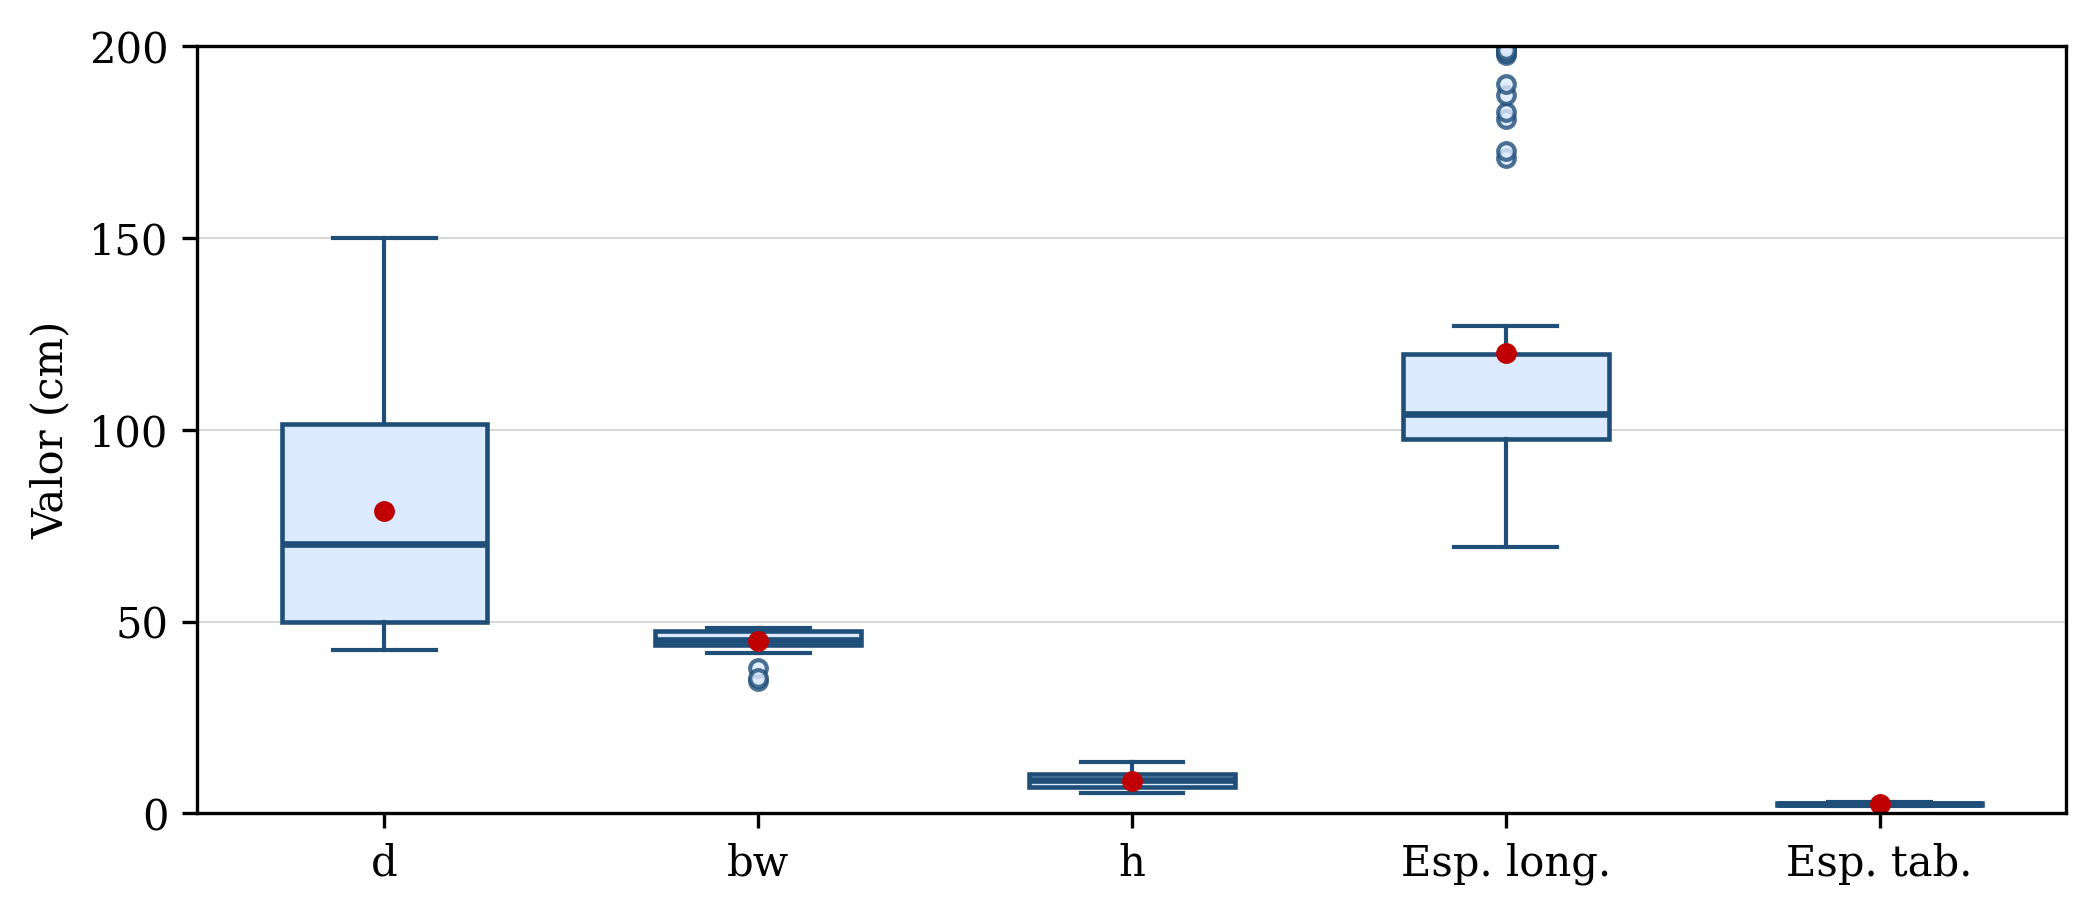
\includegraphics[width=0.75\textwidth]{figuras/boxplot_variaveis_C13.png}
    \caption{Dispersão das variáveis de projeto ao longo da fronteira eficiente da célula C-13.}
    \label{fig:boxplot}
\end{figure}

\begin{table}[!ht]
\caption{Estatística descritiva das variáveis de projeto na fronteira eficiente da célula C-13.\label{tab:estatistica}}
\begin{threeparttable}
\setlength{\tabcolsep}{3pt}
\begin{tabular*}{\textwidth}{@{\extracolsep{\fill}}lccccccc@{\extracolsep{\fill}}}
\toprule
Variável & Média & Desvio padrão & CV (\%) & Mínimo & Mediana & Máximo & Amplitude \\
\midrule
$d$ (cm) & \tofill{--} & \tofill{--} & \tofill{--} & \tofill{--} & \tofill{--} & \tofill{--} & \tofill{--} \\
$b_w$ (cm) & \tofill{--} & \tofill{--} & \tofill{--} & \tofill{--} & \tofill{--} & \tofill{--} & \tofill{--} \\
$h$ (cm) & \tofill{--} & \tofill{--} & \tofill{--} & \tofill{--} & \tofill{--} & \tofill{--} & \tofill{--} \\
$esp_{long}$ (cm) & \tofill{--} & \tofill{--} & \tofill{--} & \tofill{--} & \tofill{--} & \tofill{--} & \tofill{--} \\
$esp_{tab}$ (cm) & \tofill{--} & \tofill{--} & \tofill{--} & \tofill{--} & \tofill{--} & \tofill{--} & \tofill{--} \\
\bottomrule
\end{tabular*}
\begin{tablenotes}
\footnotesize
\item Estatísticas calculadas sobre o conjunto de soluções não dominadas da fronteira final. A plataforma exporta esta tabela automaticamente.
\end{tablenotes}
\end{threeparttable}
\end{table}

\begin{fillblock}
\noindent\textbf{[A PREENCHER]} Discutir a Figura~\ref{fig:boxplot} e a Tabela~\ref{tab:estatistica}: identificar qual variável apresenta o menor intervalo interquartil, indicando que a fronteira converge para valores praticamente fixos dessa variável independentemente do ponto escolhido pelo projetista, e qual apresenta a maior dispersão, indicando que grande parte do compromisso entre os dois objetivos é obtida ajustando essa variável. Relacionar a variável de maior dispersão com a de maior $S_{T_i}$ da Seção~\ref{sec:sobol}: se coincidirem, trata-se da variável de decisão central do problema e isso deve ser dito explicitamente; se não coincidirem, discutir a razão, pois sensibilidade e amplitude de variação são propriedades distintas.
\end{fillblock}

\subsection{Varredura paramétrica: efeito do vão e da classe de resistência}\label{sec:varredura}

Esta seção reporta o resultado das vinte células da matriz. Para cada célula, extraiu-se da fronteira eficiente a solução de menor volume de madeira, por ser a de interesse imediato para o anteprojeto, e registraram-se as dimensões correspondentes, o volume total, a flecha adimensional e a verificação governante. Os resultados consolidados constam da Tabela~\ref{tab:resultados_matriz}.

\begin{table}[!ht]
\caption{Resultados consolidados da varredura paramétrica: solução de menor volume de madeira em cada célula da matriz.\label{tab:resultados_matriz}}
\begin{threeparttable}
\footnotesize
\setlength{\tabcolsep}{3pt}
\begin{tabular*}{\textwidth}{@{\extracolsep{\fill}}llrrrrrrrl@{\extracolsep{\fill}}}
\toprule
Célula & $L$ (m) / Classe & $d$ & $b_w$ & $h$ & $esp_{long}$ & $esp_{tab}$ & $V_{\mathrm{total}}$ & $\delta_{\mathrm{tot}}/(L/250)$ & Verificação \\
 & & (cm) & (cm) & (cm) & (cm) & (cm) & (m\textsuperscript{3}) & & governante \\
\midrule
C-01 & 3{,}0 / D20 & \tofill{--} & \tofill{--} & \tofill{--} & \tofill{--} & \tofill{--} & \tofill{--} & \tofill{--} & \tofill{--} \\
C-02 & 3{,}0 / D30 & \tofill{--} & \tofill{--} & \tofill{--} & \tofill{--} & \tofill{--} & \tofill{--} & \tofill{--} & \tofill{--} \\
C-03 & 3{,}0 / D40 & \tofill{--} & \tofill{--} & \tofill{--} & \tofill{--} & \tofill{--} & \tofill{--} & \tofill{--} & \tofill{--} \\
C-04 & 3{,}0 / D50 & \tofill{--} & \tofill{--} & \tofill{--} & \tofill{--} & \tofill{--} & \tofill{--} & \tofill{--} & \tofill{--} \\
C-05 & 3{,}0 / D60 & \tofill{--} & \tofill{--} & \tofill{--} & \tofill{--} & \tofill{--} & \tofill{--} & \tofill{--} & \tofill{--} \\
\midrule
C-06 & 4{,}0 / D20 & \tofill{--} & \tofill{--} & \tofill{--} & \tofill{--} & \tofill{--} & \tofill{--} & \tofill{--} & \tofill{--} \\
C-07 & 4{,}0 / D30 & \tofill{--} & \tofill{--} & \tofill{--} & \tofill{--} & \tofill{--} & \tofill{--} & \tofill{--} & \tofill{--} \\
C-08 & 4{,}0 / D40 & \tofill{--} & \tofill{--} & \tofill{--} & \tofill{--} & \tofill{--} & \tofill{--} & \tofill{--} & \tofill{--} \\
C-09 & 4{,}0 / D50 & \tofill{--} & \tofill{--} & \tofill{--} & \tofill{--} & \tofill{--} & \tofill{--} & \tofill{--} & \tofill{--} \\
C-10 & 4{,}0 / D60 & \tofill{--} & \tofill{--} & \tofill{--} & \tofill{--} & \tofill{--} & \tofill{--} & \tofill{--} & \tofill{--} \\
\midrule
C-11 & 5{,}0 / D20 & \tofill{--} & \tofill{--} & \tofill{--} & \tofill{--} & \tofill{--} & \tofill{--} & \tofill{--} & \tofill{--} \\
C-12 & 5{,}0 / D30 & \tofill{--} & \tofill{--} & \tofill{--} & \tofill{--} & \tofill{--} & \tofill{--} & \tofill{--} & \tofill{--} \\
C-13 & 5{,}0 / D40 & \tofill{--} & \tofill{--} & \tofill{--} & \tofill{--} & \tofill{--} & \tofill{--} & \tofill{--} & \tofill{--} \\
C-14 & 5{,}0 / D50 & \tofill{--} & \tofill{--} & \tofill{--} & \tofill{--} & \tofill{--} & \tofill{--} & \tofill{--} & \tofill{--} \\
C-15 & 5{,}0 / D60 & \tofill{--} & \tofill{--} & \tofill{--} & \tofill{--} & \tofill{--} & \tofill{--} & \tofill{--} & \tofill{--} \\
\midrule
C-16 & 6{,}0 / D20 & \tofill{--} & \tofill{--} & \tofill{--} & \tofill{--} & \tofill{--} & \tofill{--} & \tofill{--} & \tofill{--} \\
C-17 & 6{,}0 / D30 & \tofill{--} & \tofill{--} & \tofill{--} & \tofill{--} & \tofill{--} & \tofill{--} & \tofill{--} & \tofill{--} \\
C-18 & 6{,}0 / D40 & \tofill{--} & \tofill{--} & \tofill{--} & \tofill{--} & \tofill{--} & \tofill{--} & \tofill{--} & \tofill{--} \\
C-19 & 6{,}0 / D50 & \tofill{--} & \tofill{--} & \tofill{--} & \tofill{--} & \tofill{--} & \tofill{--} & \tofill{--} & \tofill{--} \\
C-20 & 6{,}0 / D60 & \tofill{--} & \tofill{--} & \tofill{--} & \tofill{--} & \tofill{--} & \tofill{--} & \tofill{--} & \tofill{--} \\
\bottomrule
\end{tabular*}
\begin{tablenotes}
\footnotesize
\item Todas as células com $\rho = 5\%$ e os parâmetros de algoritmo da Tabela~\ref{tab:nsga2}. A coluna ``Verificação governante'' registra a restrição com maior valor de $g_j$ na solução reportada, isto é, a que está mais próxima do limite normativo.
\item \tofill{[A PREENCHER] Caso alguma célula não apresente solução viável -- situação plausível para as classes de menor resistência nos maiores vãos --, registrar explicitamente ``inviável'' na linha correspondente. Trata-se de resultado legítimo e informativo, que delimita o campo de aplicação da madeira de baixa classe em pontes vicinais, e não deve ser omitido da tabela.}
\end{tablenotes}
\end{threeparttable}
\end{table}

\begin{fillblock}
\noindent\textbf{[A PREENCHER]} Discutir a Tabela~\ref{tab:resultados_matriz} em três frentes.

\textbf{(i) Efeito do vão.} Quantificar o crescimento do volume de madeira com o vão, para cada classe. Como a utilização da flecha cresce aproximadamente com $L^2$ enquanto a utilização da flexão cresce com $L$, espera-se que o crescimento do consumo seja mais que proporcional ao vão. Verificar se isso se confirma e reportar o expoente aproximado, obtido por ajuste de uma lei de potência $V \propto L^{n}$.

\textbf{(ii) Efeito da classe de resistência.} Quantificar a redução de volume ao subir de classe, para cada vão. Atenção ao ponto central: a densidade cresce de 500 a 1000~kg/m\textsuperscript{3} entre D20 e D60, ou seja, dobra, enquanto a resistência à flexão triplica e o módulo de elasticidade quase dobra. Como o peso próprio é proporcional à densidade e entra na flecha, o ganho de subir de classe tende a ser decrescente e pode até se anular nos maiores vãos. Verificar se existe uma classe a partir da qual o ganho deixa de compensar, e reportar essa classe ótima por vão, caso exista. Este é o achado de maior valor prático desta seção.

\textbf{(iii) Migração da verificação governante.} Construir, a partir da última coluna, o mapa de qual verificação governa em cada região da matriz. Espera-se que o cisalhamento governe nos vãos menores, onde o esforço cortante é relativamente mais importante, e que a flecha passe a governar nos vãos maiores. Se a transição ocorrer dentro da faixa estudada, ela deve ser destacada, pois implica que a propriedade do material que importa muda ao longo da faixa de vãos: resistência nos vãos curtos, rigidez nos vãos longos.
\end{fillblock}

\subsection{Ábacos de anteprojeto}\label{sec:abacos}

Os resultados da Tabela~\ref{tab:resultados_matriz} foram convertidos em ábacos de consulta direta, destinados ao uso do projetista na etapa de concepção, antes de qualquer processamento computacional. A Figura~\ref{fig:abaco_volume} apresenta o volume total de madeira em função do vão, com uma curva por classe de resistência; a Figura~\ref{fig:abaco_volume_m2} normaliza esse volume pela área de tabuleiro, permitindo comparação direta entre vãos; e a Figura~\ref{fig:abaco_diametro} fornece o diâmetro de longarina requerido, que é a informação de aquisição mais imediata para o construtor.

\begin{figure}[!ht]
    \centering
    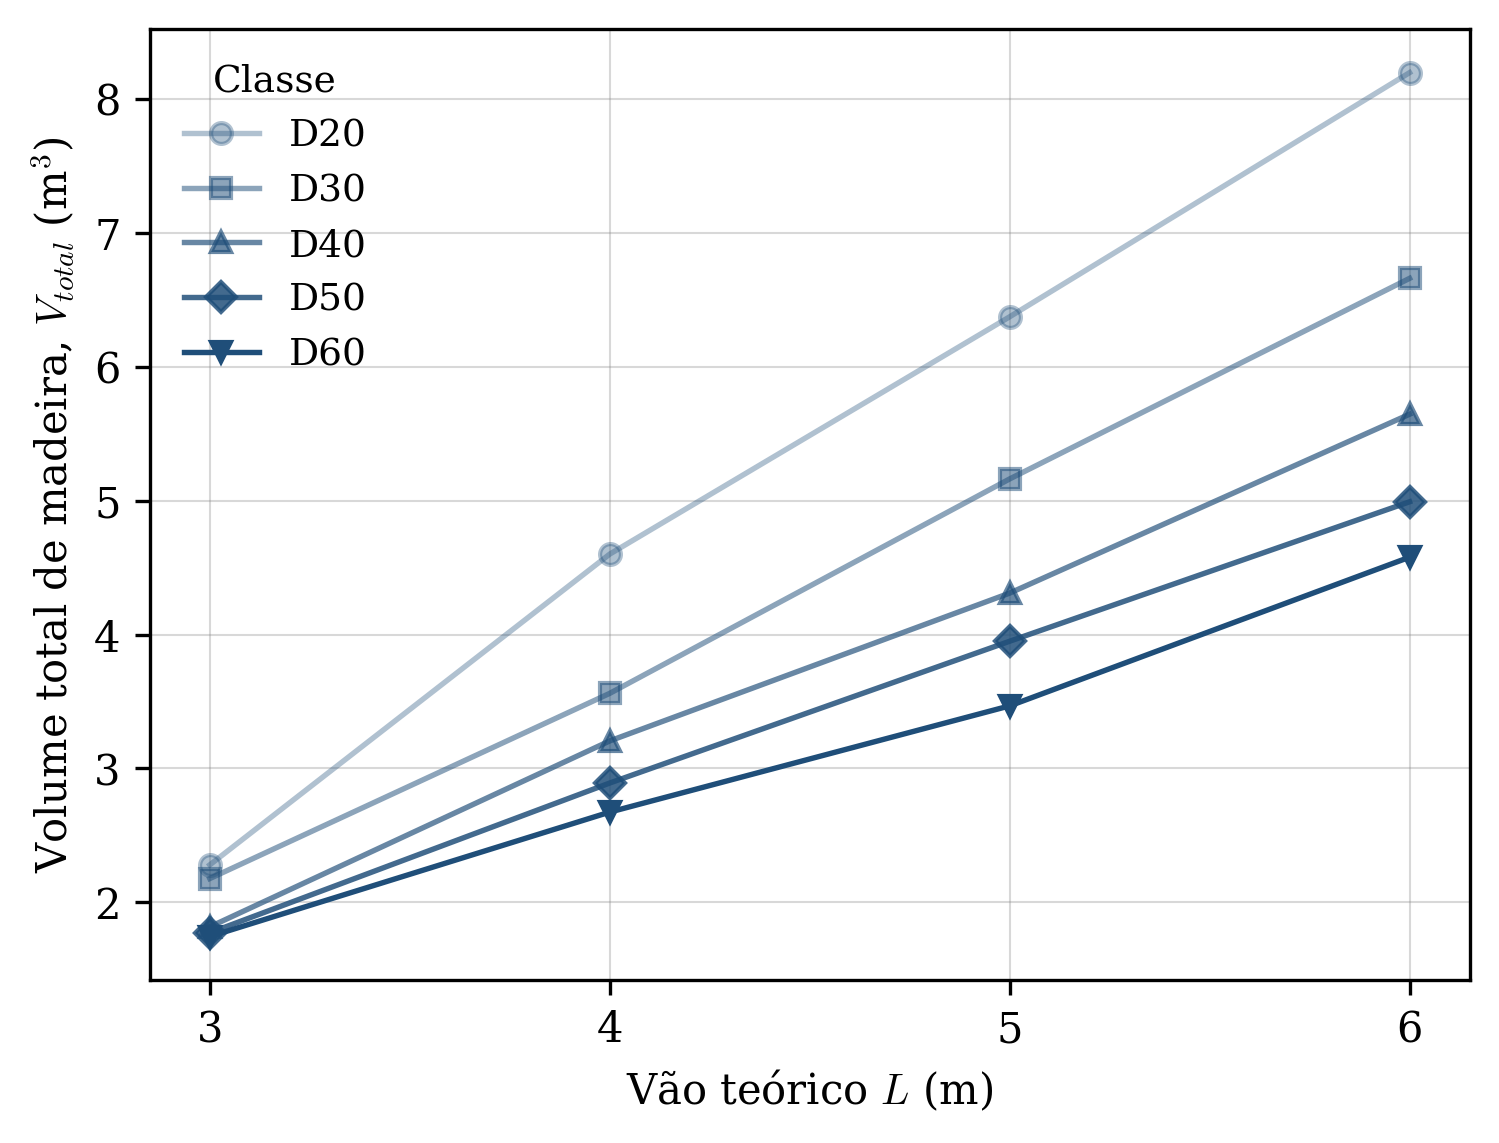
\includegraphics[width=0.7\textwidth]{figuras/abaco_volume_vs_vao.png}
    \caption{Volume total de madeira em função do vão teórico, por classe de resistência.}
    \label{fig:abaco_volume}
\end{figure}

\begin{figure}[!ht]
    \centering
    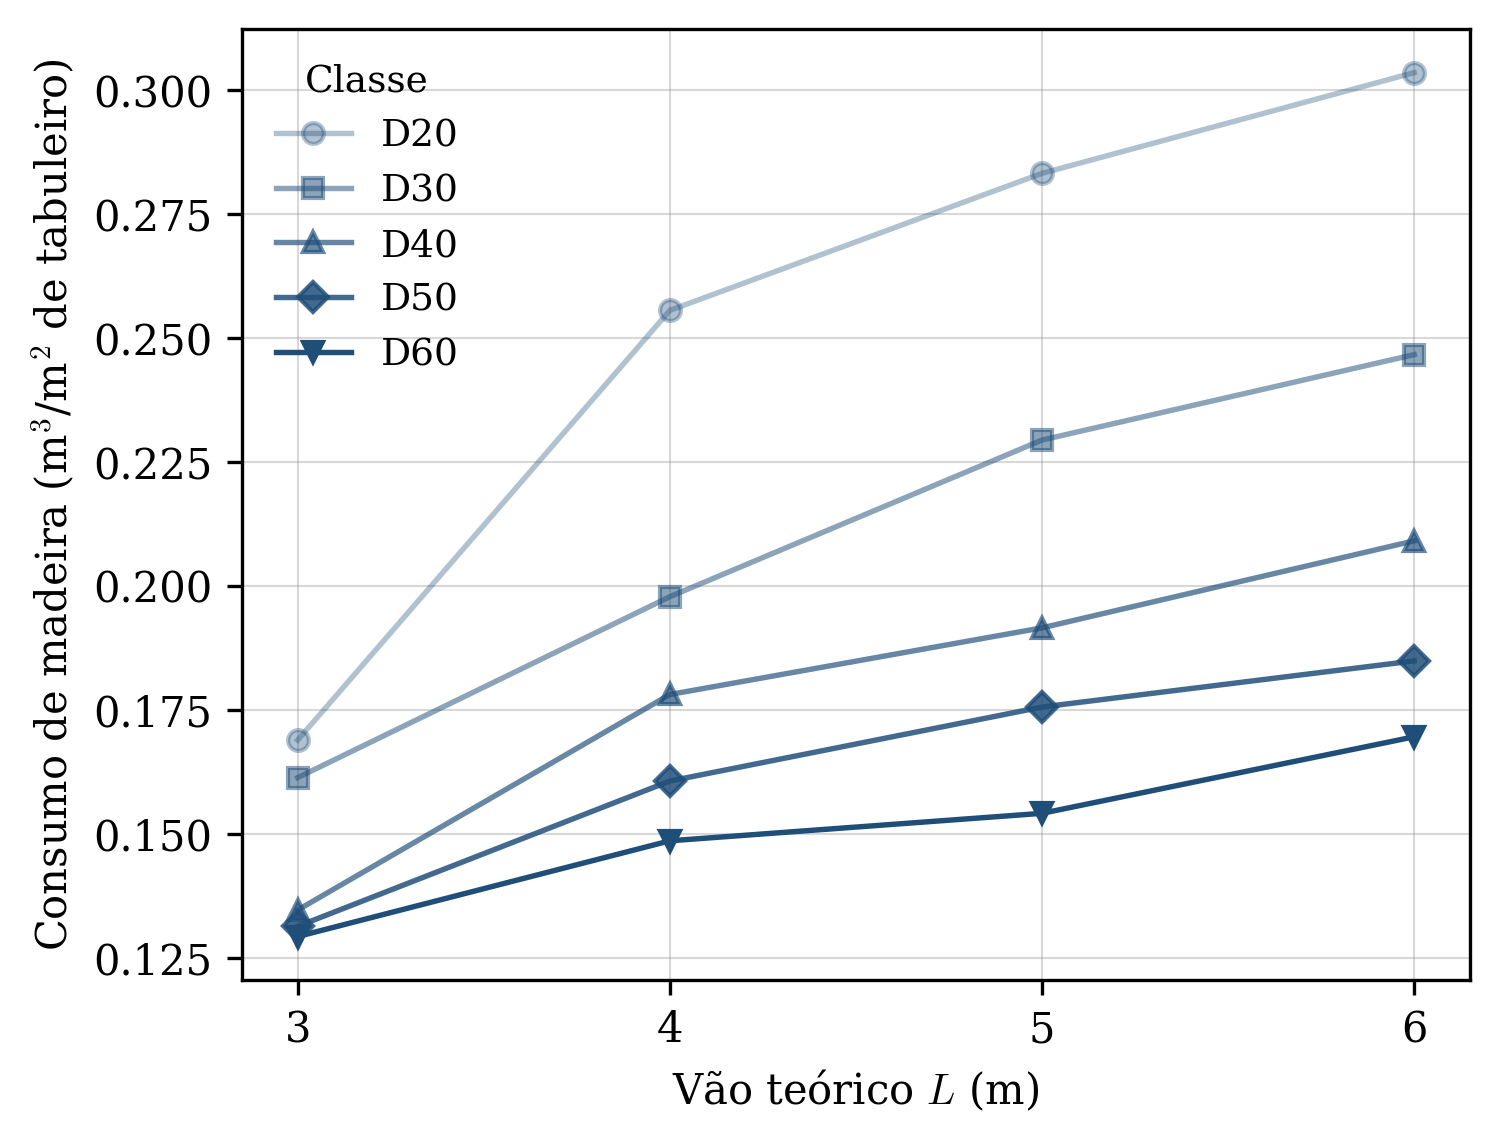
\includegraphics[width=0.7\textwidth]{figuras/abaco_volume_por_m2.png}
    \caption{Consumo de madeira por metro quadrado de tabuleiro, em função do vão teórico, por classe de resistência.}
    \label{fig:abaco_volume_m2}
\end{figure}

\begin{figure}[!ht]
    \centering
    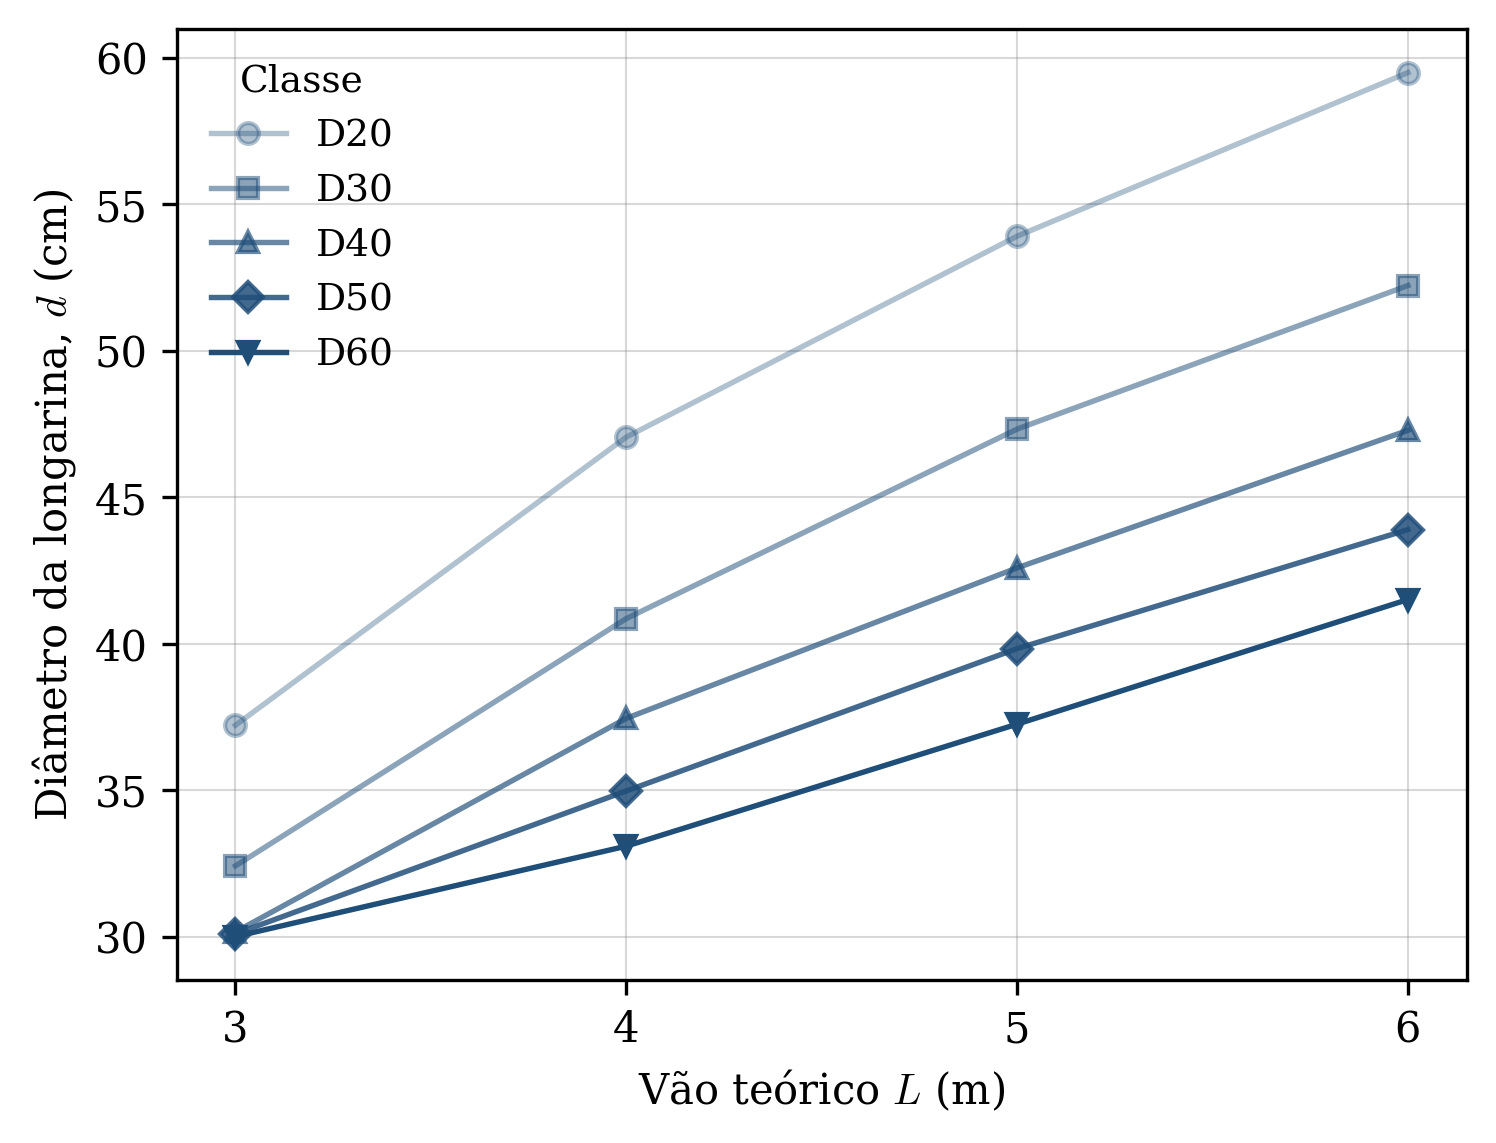
\includegraphics[width=0.7\textwidth]{figuras/abaco_diametro_vs_vao.png}
    \caption{Diâmetro de longarina requerido em função do vão teórico, por classe de resistência.}
    \label{fig:abaco_diametro}
\end{figure}

\begin{fillblock}
\noindent\textbf{[A PREENCHER]} Redigir o parágrafo de uso dos ábacos, na forma de um roteiro curto para o projetista: entrar com o vão a vencer, escolher a curva da classe de resistência da madeira disponível na região, ler o consumo esperado e o diâmetro requerido, e usar esses valores como ponto de partida para a verificação detalhada na plataforma. Explicitar as condições de validade, que são as da Tabela~\ref{tab:parametros}: pista simples de 4{,}5~m, trem tipo TB-240, classe de umidade 1, carregamento de longa duração e desvio de robustez de 5\%. Alertar que os ábacos não substituem a verificação, apenas a antecipam.
\end{fillblock}
